%%%%%%%%%%%%%%%%%%%%%%%%%%%%%%%%%%%%%%%%%%%%%%%%%%%%%%%%%%%%%%%%%%%%%%%%%%%%%%

\documentclass{l3deliverable}

%%%%%%%%%%%%%%%%%%%%%%%%%%%%%%%%%%%%%%%%%%%%%%%%%%%%%%%%%%%%%%%%%%%%%%%%%%%%%%


%%%%%%%%%%%%%%%%%%%%%%%%%%%%%%%%%%%%%%%%%%%%%%%%%%%%%%%%%%%%%%%%%%%%%%%%%%%%%%
% a utility environment for formatting tasks - see document for usage
\usepackage{tabulary}
\newenvironment{PSDTask}[2]{
  \tabularx{\linewidth}{|l|X|} \hline
    \bf\itshape Task #1: & \bf\itshape #2 \\\hline
}{\endtabularx}

\newcommand{\PSDTaskComponent}[2]{\it #1: & #2 \\ \hline}
\newcommand{\PSDTaskDescription}[1]{\PSDTaskComponent{Description}{#1}}
\newcommand{\PSDTaskOutcomes}[1]{\PSDTaskComponent{Outcomes}{#1}}
\newcommand{\PSDTaskDeliverables}[1]{\PSDTaskComponent{Deliverables}{#1}}
\newcommand{\PSDTaskRisks}[1]{\PSDTaskComponent{Risk}{#1}}

%%%%%%%%%%%%%%%%%%%%%%%%%%%%%%%%%%%%%%%%%%%%%%%%%%%%%%%%%%%%%%%%%%%%%%%%%%%%%%

\usepackage{url}

%%%%%%%%%%%%%%%%%%%%%%%%%%%%%%%%%%%%%%%%%%%%%%%%%%%%%%%%%%%%%%%%%%%%%%%%%%%%%%
%% Check these macro values for appropriateness for your own document.

\title{Project Plan}

%%authors
\author{
  Ross Adam \\
  Andrew Gardner \\
  Nicole Kearns \\
  Mamas Nicolau \\
  Asset Sarsengaliyev \\
  }

%%release date
\date{29 November 2012}

\deliverableID{D2}
\project{PSD Group Exercise 1}
\team{V}
\version{2.0}

%%%%%%%%%%%%%%%%%%%%%%%%%%%%%%%%%%%%%%%%%%%%%%%%%%%%%%%%%%%%%%%%%%%%%%%%%%%%%%

\begin{document}

%%%%%%%%%%%%%%%%%%%%%%%%%%%%%%%%%%%%%%%%%%%%%%%%%%%%%%%%%%%%%%%%%%%%%%%%%%%%%%

\maketitle

\tableofcontents

\newpage

%%%%%%%%%%%%%%%%%%%%%%%%%%%%%%%%%%%%%%%%%%%%%%%%%%%%%%%%%%%%%%%%%%%%%%%%%%%%%%
%% Standard section for all documents

\section{Introduction}

\subsection{Identification}

Project plan for the internship management system for Team V's PSD3 team project.

\subsection{Related Documentation}

{{PSD3 Group Exercise Description \url{http://fims.moodle.gla.ac.uk/file.php/128/coursework/psd3-ge-1-rev3278.pdf}}\\

Deliverables Template \url{http://fims.moodle.gla.ac.uk/file.php/128/coursework/templates.zip}\\

PSD3 Course Notes \url{http://fims.moodle.gla.ac.uk/file.php/128/lecture-notes/notes-r3275.pdf}\\

\subsection{Purpose and Description of Document}

The purpose of this document is to detail and explain the tasks which will be involved in the development of the internship management system and to identify and explain any risks which may be involved.

\subsection{Document Status and Schedule}

\begin{center}{
\begin{tabular}{|c|c|c|c|}
\hline \textbf{Date} &\textbf{Change} & \textbf{Version} & \textbf{Author}\\ 
\hline 02/10/2012 & Began Draft & 0.1 & All \\ 
\hline 09/10/2012 & Initial Draft Completed & 0.2 & All \\ 
\hline 10/10/2012 & Finalised for Submission & 0.3 & All\\ 
\hline 11/10/2012 & \textbf{Draft Submission Deadline} & 1.0 & All\\ 
\hline
\hline 26/11/2012 & Completed introduction section & 1.1 & All\\
\hline 26/11/2012 & Modified and Added Tasks & 1.2 & All\\ 
\hline 27/11/2012 & Modified and Added Tasks & 1.3 & Nicole Kearns\\
\hline 27/11/2012 & Added a Pert Chart in section& 1.4 & Mamas Nicolaou\\
\hline 28/11/2012 & Added a Gant Chart in section& 1.5 & Ross Adam\\
\hline 28/11/2012 & Modified Risk Managements Plans&1.6 & Asset Sarsengaliyev\\
\hline 28/11/2012 & Added the tasks table to section& 1.7&Mamas Nicolaou\\
\hline 28/11/2012 & Finalised for Submission &2.0& All\\
\hline 29/11/2012 & \textbf{Final Submission Deadline} &2.0  & All\\ 
\hline 
\end{tabular} }
\end{center}

%%%%%%%%%%%%%%%%%%%%%%%%%%%%%%%%%%%%%%%%%%%%%%%%%%%%%%%%%%%%%%%%%%%%%%%%%%%%%%

\section{Resources, Budgets, Schedules and Organisation}

%%%%%%%%%%%%%%%%%%%%%%%%%%%%%%%%%%%%%%%%%%%%%%%%%%%%%%%%%%%%%%%%%%%%%%%%%%%%%%

\subsection{Work Breakdown Structure}

\begin{PSDTask}{1}{Breakdown of Initial Problem Definition}
  \PSDTaskDescription{ Discussing the initial problems and forming our own ideas of how to approach the client's task.}%
  \PSDTaskOutcomes{Problem breakdown}%
  \PSDTaskDeliverables{None}%
  \PSDTaskRisks{R1}
\end{PSDTask}

\begin{PSDTask}{2}{Identify Initial Requirements}
  \PSDTaskDescription{ Using the initial problem definition, identify what the basic features of the system should be.}%
  \PSDTaskOutcomes{Inital requirements list}%
  \PSDTaskDeliverables{None}%
  \PSDTaskRisks{R1}
\end{PSDTask}

\begin{PSDTask}{3}{Prepare Interview Plan}
  \PSDTaskDescription{ Construct questions for Customer Liaison to ask the client in order to elicit requirements. Questions will then be approved by the group. An interview plan will then be written consisting of these questions.}%
  \PSDTaskOutcomes{Interview Plan document}%
  \PSDTaskDeliverables{None}%
  \PSDTaskRisks{R2}
\end{PSDTask}

\begin{PSDTask}{4}{Conduct Interview}
  \PSDTaskDescription{ Meeting with client to collect requirements using the Interview Plan document. If additional information is revealed, plan document will be deviated from.}%
  \PSDTaskOutcomes{Interview notes \& system requirements}%
  \PSDTaskDeliverables{None}%
  \PSDTaskRisks{R3}
\end{PSDTask}

\begin{PSDTask}{5}{Review Interview Notes}
  \PSDTaskDescription{Look over the notes gathered in the interview with the client and the initial requirements.}%
  \PSDTaskOutcomes{Enhanced understanding of requirements}%
  \PSDTaskDeliverables{None}%
  \PSDTaskRisks{R1, R3}
\end{PSDTask}

\begin{PSDTask}{6}{Produce Requirements Post Interview}
  \PSDTaskDescription{Produce a document containing all requirements gathered for the system from the client interview.}%
  \PSDTaskOutcomes{Requirements Document}%
  \PSDTaskDeliverables{None}%
  \PSDTaskRisks{R1, R3}
\end{PSDTask}

\begin{PSDTask}{7}{Review Initial Requirements}
  \PSDTaskDescription{Check over the requirements document to ensure it contains all requirements for the system and that they are appropriate.}%
  \PSDTaskOutcomes{Improved Requirements Document}%
  \PSDTaskDeliverables{None}%
  \PSDTaskRisks{}
\end{PSDTask}

\begin{PSDTask}{8}{Create UML Diagram of Internship Management System}
  \PSDTaskDescription{Produce a UML diagram of the system to show the structure of the internship system.}%
  \PSDTaskOutcomes{UML Diagram}%
  \PSDTaskDeliverables{D3}%
  \PSDTaskRisks{R6}
\end{PSDTask}

\begin{PSDTask}{9}{Create Use Cases}
  \PSDTaskDescription{For each of the requirements gathered, produce a use case containing all appropriate information. i.e. description, actors \& conditions}%
  \PSDTaskOutcomes{Use Cases}%
  \PSDTaskDeliverables{D3}%
  \PSDTaskRisks{R1}
\end{PSDTask}

\begin{PSDTask}{10}{Create Use Case Diagrams}
  \PSDTaskDescription{ Produce use case diagrams to show the relationship between different use cases and the actors involved.}%
  \PSDTaskOutcomes{Use Case Diagrams}%
  \PSDTaskDeliverables{D3}%
  \PSDTaskRisks{R1, R6}
\end{PSDTask}

\begin{PSDTask}{11}{Prepare Stakeholders Panel Interview Questions}
  \PSDTaskDescription{Come up with a few key questions concerning the system requirements to clarify what we are unsure of.}%
  \PSDTaskOutcomes{Stakeholder panel questions}%
  \PSDTaskDeliverables{None}%
  \PSDTaskRisks{R2}
\end{PSDTask}

\begin{PSDTask}{12}{Attend Stakeholders Panel Interview}
  \PSDTaskDescription{Allows the teams to ask further questions about the system that were not made clear in the interview.}%
  \PSDTaskOutcomes{Stakeholder panel notes}%
  \PSDTaskDeliverables{None}%
  \PSDTaskRisks{R3}
\end{PSDTask}

\begin{PSDTask}{13}{Review Notes from Stakeholders Panel Interview}
  \PSDTaskDescription{Go through the notes from the stakeholders panel and amend the requirements document where necessary.}%
  \PSDTaskOutcomes{Revised Requirements Document}%
  \PSDTaskDeliverables{None}%
  \PSDTaskRisks{R1, R3}
\end{PSDTask}

\begin{PSDTask}{14}{Finalise all Requirements}
  \PSDTaskDescription{Gather all requirements from the interview and the stakeholders panel and ensure that all requirements are included in the document.}%
  \PSDTaskOutcomes{Final Requirements Document}%
  \PSDTaskDeliverables{}%
  \PSDTaskRisks{}
\end{PSDTask}

\begin{PSDTask}{15}{Finalise UML Diagram of Internship Management System}
  \PSDTaskDescription{Modify the UML diagram to mirror the requirements gathered at the stakeholders panel.}%
  \PSDTaskOutcomes{Finalised UML Diagram}%
  \PSDTaskDeliverables{D3}%
  \PSDTaskRisks{}
\end{PSDTask}

\begin{PSDTask}{16}{Finalise Use Cases}
  \PSDTaskDescription{Modify use cases to mirror the requirements gathered at the stakeholders panel.}%
  \PSDTaskOutcomes{Finalised Use Cases}%
  \PSDTaskDeliverables{D3}%
  \PSDTaskRisks{}
\end{PSDTask}


\begin{PSDTask}{17}{Finalise Use Case Diagrams}
  \PSDTaskDescription{Modify the use case diagrams to mirror the requirements gathered at the stakeholders panel.}%
  \PSDTaskOutcomes{Finalised Use Case Diagrams}%
  \PSDTaskDeliverables{D3}%
  \PSDTaskRisks{}
\end{PSDTask}

\begin{PSDTask}{18}{Finalise Requirements Specification Documents}
  \PSDTaskDescription{Check over the requirements specification to ensure it is correct and contains all relevant information for the use cases and that the use case diagrams match the information in the descriptions.}%
  \PSDTaskOutcomes{Finalised Requirements Specification Documents}%
  \PSDTaskDeliverables{D3}%
  \PSDTaskRisks{}
\end{PSDTask}

\begin{PSDTask}{19}{Research Bash Scripting}
  \PSDTaskDescription{Learn how to write bash scripts in order to create a prototype to demonstrate to the client the basic functionality and workflow of the system.}%
  \PSDTaskOutcomes{Understanding of Bash Scripting}%
  \PSDTaskDeliverables{None}%
  \PSDTaskRisks{}
\end{PSDTask}

\begin{PSDTask}{20}{Create Bash Prototype}
  \PSDTaskDescription{Create a prototype of the system written in Bash scripting language.}%
  \PSDTaskOutcomes{Bash prototype}%
  \PSDTaskDeliverables{D4}%
  \PSDTaskRisks{R8}
\end{PSDTask}

\begin{PSDTask}{21}{Test Bash Prototype}
  \PSDTaskDescription{Test the prototype to ensure there are no bugs and that it works as expected.}%
  \PSDTaskOutcomes{Tested Bash prototype}%
  \PSDTaskDeliverables{D4}%
  \PSDTaskRisks{}
\end{PSDTask}

\begin{PSDTask}{22}{Demonstrate Bash Prototype to Client}
  \PSDTaskDescription{Demonstrate prototype to client allowing for questions and feedback.}%
  \PSDTaskOutcomes{Prototype demonstration \& feedback}%
  \PSDTaskDeliverables{D4}%
  \PSDTaskRisks{}
\end{PSDTask}

\begin{PSDTask}{23}{Review Feedback from Bash Prototype Demonstration}
  \PSDTaskDescription{Go through feedback from demonstration, comparing to requirements specification.}%
  \PSDTaskOutcomes{Requirements specification validation}%
  \PSDTaskDeliverables{D4}%
  \PSDTaskRisks{}
\end{PSDTask}


%%%%%%%%%%%%%%%%%%%%%%%%%%%%%%%%%%%%%%%%%%%%%%%%%%%%%%%%%%%%%%%%%%%%%%%%%%%%%%

\subsection{Resource Estimation and Allocation to WBS\label{sec:allocation}}
The available human resourses for this project are 5 developers as defined in document D1.\\
According to the tasks list (section 2.3) the total estimated duration of this WBS will be 44 hours or 6 working days.\\
\\
Resources Available:\\
\\
Andrew Gardner: Chief Architect \\
Asset Sarsengaliyev: Source Code Manager\\ 
Mamas Nicolaou: Quality Assuror \\
Nicole Kearns: Quality Assuror \\
Ross Adam: Project Manager \\
\\
Resource allocation details are shown in the Task Table below. 

%%%%%%%%%%%%%%%%%%%%%%%%%%%%%%%%%%%%%%%%%%%%%%%%%%%%%%%%%%%%%%%%%%%%%%%%%%%%%%

\subsection{Schedules}

\begin{table}
\caption{Tasks Table} % title of Table
\begin{tabular}{|c |c |c |c |c |} % centered columns (4 columns)
\hline\hline                        %inserts double horizontal lines
Task & Title & Hours & Depend & Team Members \\ [0.5ex]
\hline1 & Breakdown of Initial Problem Definition & 5:00 &-& All\\ % inserting body of the table
\hline2 &Identify Initial Requirements & 3:00 & 1 & All\\
\hline3 & &  & & Ross Adam, \\
 &  Prepare Interview Plan&3:00 &2 &Nicole Kearns, \\
 & & & &Asset Sarsengaliyev \\
\hline4 & Conduct Interview & 0:15 &3& All\\
\hline5 & Review Interview Notes& 1:00 &4& All\\
\hline6 & Produce Requirements Post Interview & 1:00 &5& All\\
\hline7 & Review Initial Requirements & 1:00 &6& All \\
\hline &  &  & &Asset Sarsengaliyev, \\
8&Create UML Diagram of Internship Management System&3:00 &7 &Nicole Kearns,  \\
& & & & Andrew Gardner \\
\hline9  & Create Use Cases & 2:00&7 &Nicole Kearns,\\
 & & & & Ross Adam \\
\hline10  & Create Use Case Diagrams &2:00 &9 &  Andrew Gardner, \\
 & & & & Mamas Nicolaou \\
\hline11 & Prepare Stakeholders Panel Interview Questions & 1:00 &7& All\\
\hline12 & Attend Stakeholders Panel Interview & 1:00 &11& All\\
\hline13 & Review Notes from Stakeholders Panel Interview & 1:00 &12& All\\
\hline14 & Finalise all Requirements & 2:00 &13& All\\
\hline15 & Finalise UML Diagram of Internship Management System & 1:00 &14& All\\
\hline & &  & & Andrew Gardner, \\
 16&Finalise Use Cases &1:00 & 14& Mamas Nicolaou, \\
 &  & & &Nicole Kearns \\
\hline&  & & & Nicole Kearns, \\
 17 & Finalise Use Case Diagrams & 1:00& 16& Ross Adam, \\
 & &  & &Mamas Nicolaou \\
\hline18 & Finalise Requirements Specification Documents & 2:00 &15,17& Ross Adam \\
\hline19 & Research Bash Scripting & 3:00 &-&Andrew Gardner\\
\hline20 & Create Bash Prototype & 6:00 &19,18&Andrew Gardner \\
\hline21 & Test Bash Prototype & 2:00 &20& Mamas Nicolaou \\
\hline22 & Demonstrate Bash Prototype to Client& 0.30 &21& All\\     
\hline23 & Review Feedback from client about Bash Prototype & 1:00 &22& All\\      
\hline %inserts single line
\end{tabular}
\label{table:nonlin} % is used to refer this table in the text
\end{table}
\pagebreak

\subsection{Pert Chart}
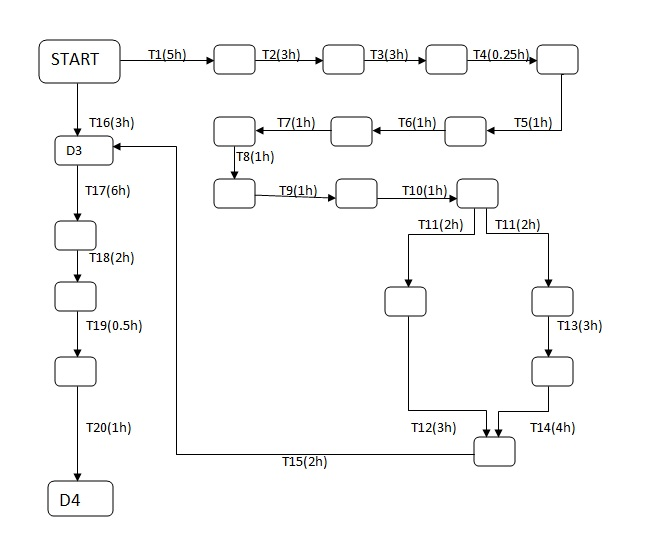
\includegraphics[scale=0.7]{img/PERT.jpg}

\subsection{Gantt Chart}

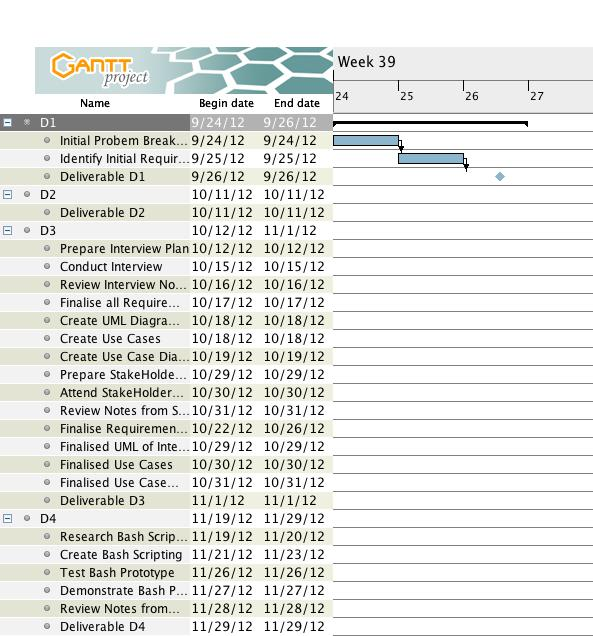
\includegraphics[scale=0.7]{img/GANTTD1.jpg}\\
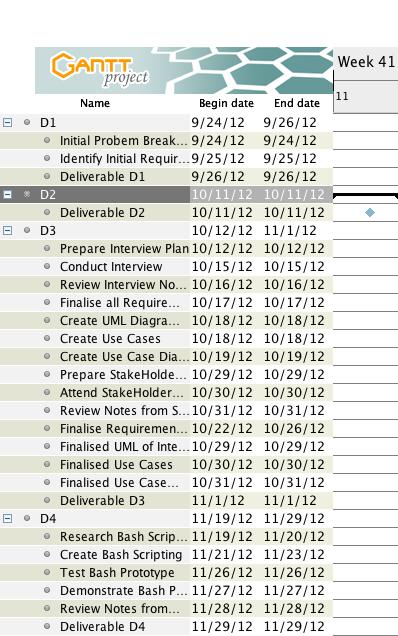
\includegraphics[scale=0.7]{img/GANTTD2.jpg}\\
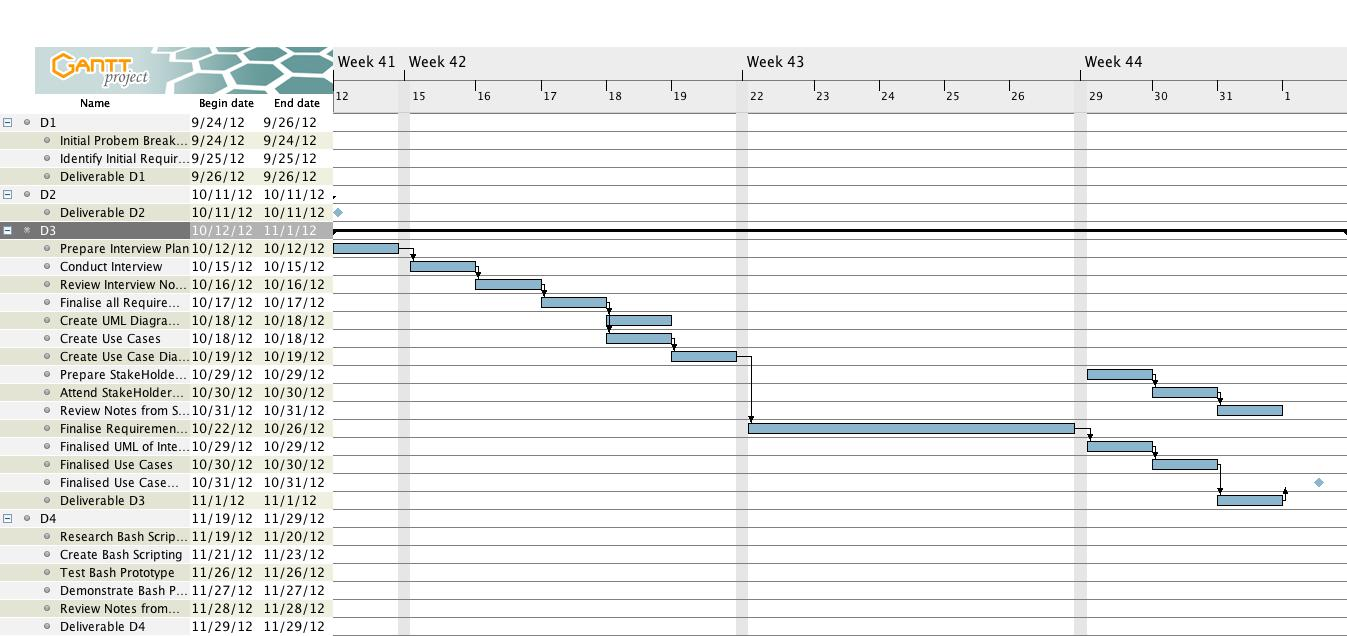
\includegraphics[scale=0.3]{img/GANTTD3.jpg}\\
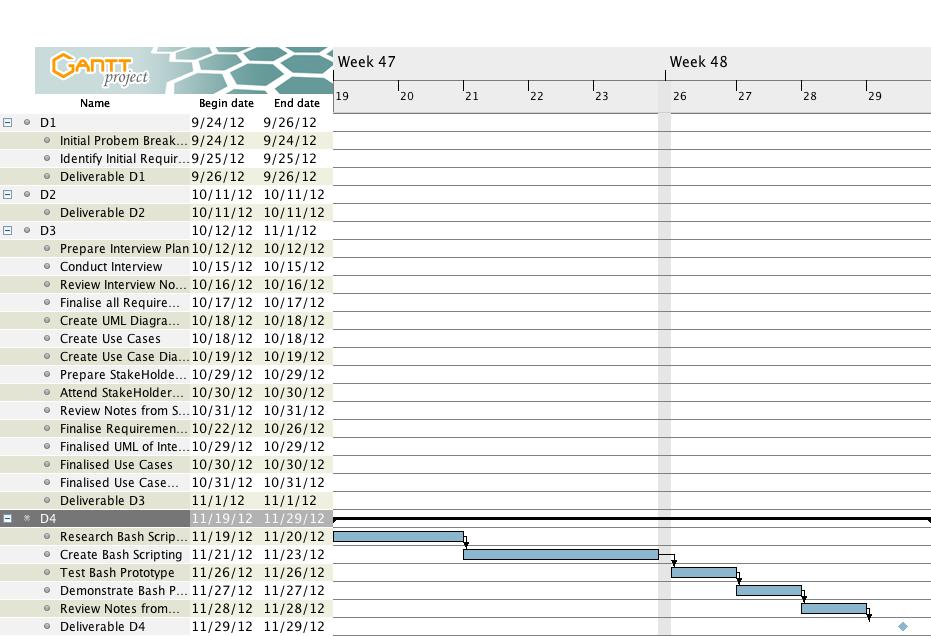
\includegraphics[scale=0.5]{img/GANTTD4.jpg}\\



%%%%%%%%%%%%%%%%%%%%%%%%%%%%%%%%%%%%%%%%%%%%%%%%%%%%%%%%%%%%%%%%%%%%%%%%%%%%%%

\subsection{Equipment, Materials, Facilities, and Other Resources}
\textbf{Equipment:} Level 7 Dell Lab Machines\\
\textbf{Materials:} Pen \& paper\\
\textbf{Facilities:} Boyd Orr Building's Level 7 Computing Lab\\

%%%%%%%%%%%%%%%%%%%%%%%%%%%%%%%%%%%%%%%%%%%%%%%%%%%%%%%%%%%%%%%%%%%%%%%%%%%%%%

\section{Quality Assurance Plan}


The Quality Assurance Plan is the basis for maintaining the quality of our product on the highest level that matches the requirements for the given software system and approved by stakeholders. The QAP will be overseen by the team to maintain quality improvement activities, such as monitoring, adding features and evaluating defects. The purpose of the QAP is designed to match the following requirements:\\

\begin{itemize}
\item to perform suitable actions when possibilities for improvements in service are identified.\\
\item to implement corrective action when technical issues or bugs are found.\\
\item to ensure that the software system is maintaining properly all the time.\\
\end{itemize}

Our team will mainly rely on Risk Management Plan, Product Requirements Specification and Change Management Plan to keep the product quality to the appropriate level.\\

Team activities:\\

Team members use the special group on Facebook to discuss their thoughts. All the documentation and code are  accessible on GitHub for all members as well as supervisors. It is the responsibility of everyone to ensure that update will not harm any working parts of the system. After altering any part of the code, we invoke test sets to check if the corresponding oracles match expected outputs.\\ 

Team should have one or more meetings every week to discuss the progress of the work. The tasks should be equally divided by team members and this is being added to the timeline of tasks. Every member is in charge of reviewing all finished tasks and task is approved by team if two or more member of the team approves it. \\

Product documentation(Deliverables) are ready to submit when members have no offers how to improve the document. Latex tool is used to produce the documentation.  Feedback for the deliverables is carefully analysed and corrections are done by the whole team at the end of term.\\

In order to make sure the quality of the product will be high and the team is in the right direction, team meets the supervisor every week as well as the clients few times per term.\\

Apart from that, we use black box testing with other teams to check if they can find bugs in prototype, as they have a fresh look to the product.\\

%%%%%%%%%%%%%%%%%%%%%%%%%%%%%%%%%%%%%%%%%%%%%%%%%%%%%%%%%%%%%%%%%%%%%%%%%%%%%%

\section{Risk Management Plan}

\begin{center}{
\begin{tabular}{|p{2cm}|p{2cm}|p{3cm}|p{2cm}|p{3cm}|p{2cm}|}
\hline \textbf{Risk ID} &\textbf{Category} & \textbf{Description} & \textbf{Probability} & \textbf{Impact} & \textbf{Controls}\\
\hline R1 & Requirements & Functional and non-functional requirements may be interpreted differently by team members due to the lack of interviews. & Meduim & High / The final product may behave differently and delays in fixing problems. & C1, C3, C5\\
\hline R2 & Requirements & Team members may ask inappropriate questions or miss important requirements. & Low & Medium / This may lead to improper documentation of the product. & C2, C8\\
\hline R3 & Requirements & The stakeholders are not sure how the final product should be. & High & Medium / Stakeholders may not be satisfied with product developed. & C1, C3, C5\\
\hline R4 & Skills & Team Members may overestimate their skills & Very high & Medium / The quality of the product will be lower than what was specified. & C1, C3, C5\\
\hline R5 & Requirements & Releasing poorly written documents to the client. & Medium & High / Consequently, the product may not reach expectations & C3, C5, C7\\
\hline R6 & Technical & Team members are unfamiliar with appropriate tools & Medium & High/ Consequently, the product may not reach expectations & C3, C7\\
\hline R7 & Requirements & Tasks may be left from the time-line & Medium & Medium/ This may lead to potential delays & C6\\
\hline R8 & Prototyping & Prototype is not compatible with client's specification & Medium & High/ Changing all specification and possibly start all the work again & C3, C7\\
\hline
\end{tabular} }
\end{center}

\begin{center}{
\begin{tabular}{|c|c|}
\hline \textbf{Control ID} & \textbf{Description}\\
\hline C1 &  Iteratively checking the specification of the product with stakeholders\\
\hline C2 & Prepare the questions with team for the interview\\
\hline C3 & Use other expert advise about the product development\\
\hline C4 & Make presentation of the software system to the stakeholders\\
\hline C5 & Develop the prototype of the product, based on bash script\\
\hline C6 & Check the work by two members of the team\\
\hline C7 & Investigate software competency and other skills within team\\
\hline C8 & Assign one member to conduct the interviews\\
\hline
\end{tabular} }
\end{center}

%%%%%%%%%%%%%%%%%%%%%%%%%%%%%%%%%%%%%%%%%%%%%%%%%%%%%%%%%%%%%%%%%%%%%%%%%%%%%%

\section{Configuration Management Plan}

To safely and successfully produce both the documentation and code
associated with our program there must be a stringent configuration
management plan.\\

\begin {enumerate}
\item \textbf{Change Management}\\
The decision to create a prototype rather than use incremental
development will allow us to let the client interact with a primitive,
yet functional system quickly.\\
The prototype will help elicit and validate system requirements while
also increasing our understanding of the system and uncover any
additional requirements that may have been omitted.\\

\item \textbf{Version Management}\\
In order to prevent a team member's work being overwritten
accidentally, Team V will be using GitHub to keep a central repository
of work. This can then be pulled from the GitHub site and worked on in
a local workspace. To prevent the aforementioned interference, local work is
merged back into the central repository safely.\\  

\item \textbf{System Building}\\
As above we will be using GitHub to maintain consistency in the
codeline.\\

\item \textbf{Release Management}\\
Team V will be utilising the issues feature on GitHub to highlight
completed tasks and milestones. It can also be used to assign new
tasks for memebers to complete. This will allow the team to track
current releases. \\
\end{enumerate}

Generally, if changes need to be made the team will have to discuss
several different points to conclude if it should be addressed:\\

\begin{enumerate}
\item \textbf{Consequences of not implementing the change}\\
If a change is needed to alter a serious system failure it will be
prioritised and addressed quickly. However, if it is a simple error it
will be logged and corrected as current high priority tasks allow.

\item \textbf{Benefits of change}\\
Will the change benefit the majority of users or will it simply
benefit the change proposer.

\item \textbf{Number of Users affected by change}\\
If the change is for the benefit of only a few users is it worth the
risk to potentially adversely effect more users?

\item \textbf{Cost of making the change}\\
If the change is likely to create new bugs or take a lng time to
implement it may simply be rejected.

\end{enumerate}

If these steps are followed then the software can be maintained
easily and changes can be handled efficiently.

%%%%%%%%%%%%%%%%%%%%%%%%%%%%%%%%%%%%%%%%%%%%%%%%%%%%%%%%%%%%%%%%%%%%%%%%%%%%%%

\appendix

\section{Glossary}

\textbf{PSD3:} Professional Software Development 3\\
\textbf{CC:} Course Co-ordinator\\
\textbf{QAP:} Quality Assurance Plan\\

\end{document}

%%%%%%%%%%%%%%%%%%%%%%%%%%%%%%%%%%%%%%%%%%%%%%%%%%%%%%%%%%%%%%%%%%%%%%%%%%%%%%

